\documentclass[10pt, a4paper]{article}

\usepackage{amsmath}
\usepackage{amssymb}
\usepackage{fullpage}
\usepackage{algorithm2e}
\usepackage{graphicx}
\usepackage{wrapfig}



\newcounter{wssection}
\newcounter{wsexercise}[wssection]


\newcommand{\worksheetsection}[1]{
\vspace{10mm}
\stepcounter{wssection}
\noindent \Large \textbf{\thewssection. #1} \normalsize
\vspace{3mm}
}


\newcommand{\worksheetexercise}{
\stepcounter{wsexercise}
\vspace{5mm} \noindent \textbf{Exercise \thewssection.\thewsexercise \;}
}


\title{Dublin R Workshop on Bayesian Data Analysis}
\author{Mick Cooney\\mickcooney@gmail.com}
\date{February 19, 2014}


\begin{document}

\maketitle

\worksheetsection{Introducing the Data and the Analysis}

\noindent
In order to learn and explore the use of Bayesian Data Analysis, we
need some kind of problem to solve, and data with which to solve
it. Before we begin, it is worth looking at the problem we are trying
to solve, exploring the data for its structure and layout, and just
getting a `feel' for the issues we may have to face.

Our problem is a little contrived, and the data has been generated
randomly, but it should be relatively straightforward to generalise
this for other problems.

Our dataset is a set of outcomes of cointosses, where the coins have
been minted from three separate mints, and we want to get an estimate
of the quality of the output from the three mints.

For the purposes of estimating and inferring on mint-quality, we are
looking for coins that are as fair as possible i.e. have a $\theta$ as
close to $0.50$ as possible, and can do so as consistently as
possible, i.e. the variance of the $\theta$ values for the coins is as
low as possible.

So, to start, we should first load the data, and then start to explore
it.

\worksheetexercise Load the data into the workspace using the code
given in \texttt{setup\_data.R}.

\worksheetexercise Using whatever summary methods you like,
investigate the mean and variance of the $\mu$ for each mint.

\worksheetexercise Use density estimation to explore the distribution
of $\theta$s for each mint.

\vspace{5mm}
\noindent
\textbf{Hint:} The code in \texttt{explore\_data.R} may be of use to get you started.


\worksheetsection{Using the Hierarchical Model in JAGS}

\noindent
We build our first JAGS model based off the data from a single
mint. Our hierarchical model is represented in Figure \ref{fig1}.

\begin{figure}[h]
\begin{center}
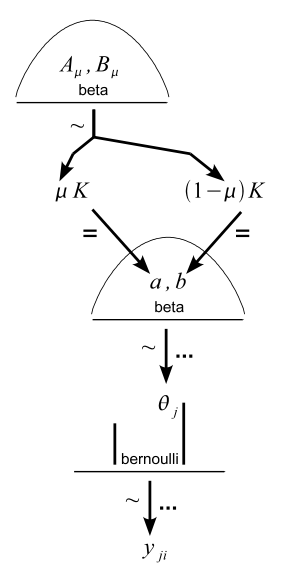
\includegraphics[height=10cm]{hierarchical_singlemint_multiplecoin.png}
\caption{\label{fig1}
Graphical Representation of the Single Mint, Single Coin Hierarchical
model}
\end{center}
\end{figure}

\vspace{5mm}

\noindent
One issue with running JAGS models is that it can take time. To help
with this issue, two `reduced' versions of the data are produced, and
this simple task raises an immediate question of how to do this.

\worksheetexercise Investigate the setup code for any sampling issues
that may arise.

\worksheetexercise Using a reduced data set, run the hierarchical code
for each mint. Compare the results.

\worksheetexercise Plot the $\mu$ and $\kappa$ for each mint in the
same plot.

\worksheetexercise Rerun the code for the other reduced dataset, and
compare with previous results.

\worksheetexercise Run the code with the full dataset, again comparing
with the two previous outputs.

\vspace{5mm}

\noindent
Since performance is always an issue, we can investigate the speedup
of switching from a Bernoulli distribution at the lowest level, to a
Binomial one. This involves a little preprocessing on the data, but
nothing too difficult.

\worksheetexercise Perform the above analysis, but using the binomial
distribution at the lowest level. Use \texttt{Sys.time()} to time to
the two runs.

\vspace{5mm}
\noindent
\textbf{Hint:} The code in \texttt{run\_bern\_singlemint.R} and
\texttt{run\_beta\_singlemint.R} may be of help here.



\worksheetsection{Expanding the Model to Compare Mints}

\noindent
While the methods employed in the previous section work fine, a more
`Bayesian' approach would be to incorporate the mint data into the
model, rather than running a separate run for each mint. As you
imagine, this is especially true if there are a large number of
separate entities at the highest hierarchy of the model.

Incorporating the mint data for each coin is relatively simple --- we
just need to index by $\mu$ and $\kappa$ for each mint, as shown in
Figure \ref{fig2}.

\begin{figure}[h]
\begin{center}
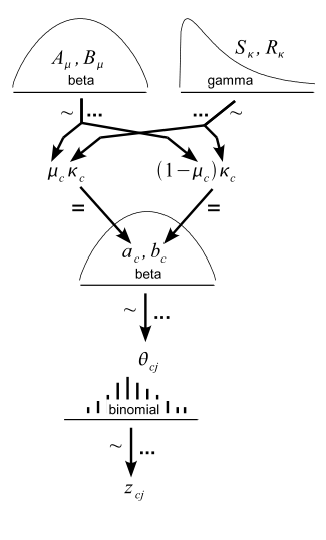
\includegraphics[height=10cm]{hierarchical_multiplemint_multiplecoin.png}
\caption{\label{fig2}
Graphical Representation of the Multiple Mint, Multiple Coin Hierarchical
model}
\end{center}
\end{figure}


\worksheetexercise Using the reduced data, run the full multiple coin,
multiple mint hierarchical model, and investigate the output.

\worksheetexercise Is there any difference in the posterior
distributions from this approach to the single mint model?

\worksheetexercise How do the above posterior distributions compare to the simple density estimation distributions we originally produced?

\vspace{5mm}
\noindent
\textbf{Hint:} The code in \texttt{run\_multiplemint.R} may be of help here.


\worksheetsection{Exploring the Effect of the Data}

\noindent
We are going to investigate the effect that the composition of the
data has on inference. This can be important if we have a constrained
amount of data collection at the lowest level, but have a certain
amount of discretion at the higher levels.

So, suppose we have a relatively fixed amount of total coin tosses we
can record, but we can choose whether to use more coins per mint, or
more tosses per coin. How does this affect the output of our analysis?

\worksheetexercise Inspect the code in the function
\texttt{generate.cointoss.data()} and make sure you understand how it
works.

\worksheetexercise Use the function to generate a dataset with a
relatively high number of coins per mint, and low number of tosses per
coin.

\worksheetexercise Use the function to generate a dataset with a
relatively high number of coins per mint, and low number of tosses per
coin.

\worksheetexercise Use all of the above to investigate the above
compositional effects of the data on the outputs of our model?



\worksheetsection{Further Work and Open Questions}


\worksheetexercise Is there ways in which we can improve the data
generation to help us understand how this approach handles differences?

\worksheetexercise How do we incorporate errors in data collection to
our model?

\worksheetexercise What kind of effects would these errors have on our
output and our conclusions?

\worksheetexercise How can we extend this model at the higher
levels?




\end{document}
